\section{BUS e protocolli}
In questa sezione presentiamo i bus e i protocolli visti a lezione inerenti all'architettura ARM utilizzata sul SoC.

\subsection{I2C}
$I^2 C$ (Inter-Integrated Circuit) è un sistema di comunicazione seriale nato negli anni '80 sincrono utilizzato tra circuiti integrati. Risponde alla problematica di ridurre il più possibile il numero di cavi in una comunicazione seriale, ed è utilizzata per interconnettere sensori ad un'architettura principale. Come tutti i sistemi seriali, è sincrono. 
Questo protocollo/bus distingue i device in \textit{Master}, che iniziano la comunicazione, e \textit{Slave}. Questo sistema prevede più device master connessi allo stesso bus. Tecnicamente prevede due segnali, uno per la trasmissione dei dati e uno per il segnale di sincronizzazione. Il limite principale di questo protocollo è la velocità di trasmissione. 

I cavi necessari sono:
\begin{itemize}
    \item SDA - Serial Data: cavo per la trasmissione dei dati;
    \item SCL - Serial Clock: cavo per la trasmissione del clock;
    \item GND - Ground comune tra dispositivi;
\end{itemize}

Ai segnali di SDA e SCL viene aggiunta una terza linea Vcc, a cui sono connessi i SDA e SCL tramite resistori di pull-up: infatti lo stato di riposo delle linee è il valore logico HIGH (figura \ref{img:i2c_logic_1}).

\begin{figure}[ht]
    \centering
    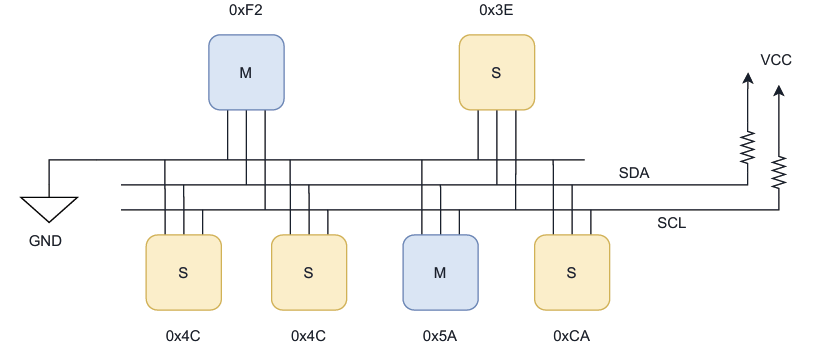
\includegraphics[width=.7\textwidth]{img/i2c_1.png}
    \caption{i2c bus - schema logico}
    \label{img:i2c_logic_1}
\end{figure}

Ogni device connesso sul bus è identificato da un indirizzo a 7 bit. L'indirizzo è assegnato al device in fase di produzione, e nella maggior parte dei casi non è modificabile. Possono tuttavia coesistere dispositivi aventi lo stesso indirizzo 

La comunicazione I2C viene inziata da un master, che comunica il bit S di \textit{START}, ovvero una transizione da alto a basso del segnale di dato mentre il clock SCL è a livello logico alto. Dopodichè, il master porta SCL a livello logico basso e impone sul segnale SDA il valore del primo bit. Dopo i transienti, il dato è stabile e può essere letto (tratto verde di figura \ref{img:i2c_logic_2}), segnalato dalla commutazione di SCL. Si continua in questo modo trasmettendo tutti gli altri bit. La transazione termina con un ottavo bit finale che indica la natura dell'operazione (Lettura o scrittura verso devices slave). Osserviamo infine che SDA vine commutato da basso ad alto quando SCL è alto. 

\begin{figure}[ht]
    \centering
    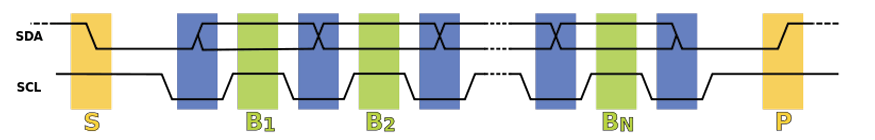
\includegraphics[width=.7\textwidth]{img/i2c_2.png}
    \caption{i2c bus - tempificazioni}
    \label{img:i2c_logic_2}
\end{figure}

Il protocollo definisci tre tipi fondamentali di transazioni, ognuna delle quali inizia con uno START e finisce con uno STOP.
\begin{itemize}
    \item messaggio singolo in cui un master scrive dati a uno slave;
    \item messaggio singolo in cui un master legge dati da uno slave;
    \item formato combinato, dove un master effettua almeno due lettura o scrittura a uno o più slave.
\end{itemize}

Dopo lo START, il master impone sul bus l'indirizzo dello slave con cui vuole comunicare. Indirizzi e dati per convenzione sono trasmessi dal bit più significativo. 
Nel caso di messaggio singolo, il master inizia lo scambio di informazioni inviando lo start bit seguito dall'indirizzo dello slave con cui vuole comunicare. Segue un ottavo bit che indica se vuole trasferire informazioni allo slave o riceverne. Se lo slave indirizzato esiste, il master prende conotrollo della linea dati sul successivo impulso alto del SCL imponendo SLC LOW. 
Se il master desidera scrivere allo slave, allora invia ripetutamente un byte con lo slave che invia un bit ACK. Se il master desidera leggere dallo slave, allora riceve ripetutamente un byte dallo slave, e invia un bit ACK dopo ogni byte tranne l'ultimo. 
Poichè il bus è multimaster e in generale è condiviso, può capitare che il bus venga conteso. Il protocollo di risuluzione adottato da I2C è deterministico: ogni trasmettitore controlla il livello della linea dati (SDA) e lo confronta con i livelli che si aspetta; se non corrispondono, quel trasmettitore ha perso l'arbitrato e abbandona questa interazione del protocollo. 

Una caratteristica fondamentale di I2C è il \textbf{Clock Stretching}: un dispositivo slave indirizzato può tenere la linea di cloack SCL bassa dove aver ricevuto o inviato un byte, indicando che non è ancora pronto ad elaborare altri dati.
Il master che sta comunicando con lo slave non può finire la trasmissione del bit corrente, ma deve aspettare che la linea di clock vada effettivamente alta. Se lo slave è in clock-stretching, la linea di clock sarà ancora bassa perchè le connessioni sono \textit{open drain}: questo significa che nessuno può forzare la linea alta, ma può solo forzarla bassa.